\documentclass[a4paper]{article}
\usepackage{listings}
\usepackage{pgf}
\usepackage[utf8]{inputenc}
\usepackage{verbatim}
\usepackage{titling}
\usepackage{booktabs}
\usepackage{enumitem}
\usepackage{qtree}
\usepackage{amssymb}
\usepackage{amsmath}
\usepackage{times}
\usepackage{dsfont}
\usepackage{titling}
\usepackage[a4paper,
bindingoffset=0.2in,
left=1in,
right=1in,
top=2in,
bottom=1in,
footskip=.25in]{geometry}
\usepackage{cite} %bibtex
\usepackage{pdfpages}

\pretitle{\begin{center}\linespread{1}}
  \posttitle{\end{center}\vspace{0.14cm}} 
\preauthor{\begin{center}\Large}
  \postauthor{\end{center}}

\setlength{\droptitle}{-10em}
\title { \Large{Seminario de Ciencias de la Computaci\'on B}\protect\\
  \large{Heurísticas de Optimización Combinatoria}\protect\\
  \large{Problema del Ajente Viajero\\con Recocido Simulado}}


\date{\normalsize{Viernes, 17 de Marzo, 2023.}}
\author{\normalsize{Profesor: Canek Peláez Valdés}\protect\\
  \normalsize{Autor: Xin Wen Zhang Liu}}\vspace{0.2cm}

\clearpage



\begin{document}
\allowdisplaybreaks
\maketitle

\subsection*{El problema del agente viajero}
El problema del agente viajero es uno de los problemas de Optimización combinatoria m\'as estudiados. Introducido por primera vez en 1930 \\

Este problema plantea una pregunta f\'acil de hacer pero dif\'icil de repsonder:
\begin{center}
  Dado un conjunto de ciudades y sus coordenadas en el plano cartesiano, ?`cu\'al es el camino m\'as corto que visite cada ciudad exactamente una vez?
\end{center}
La manera m\'a directa de resolver este problema ser\'ia listar todas las prosibles combinaciones de caminos que pasen por las ciudades deseadas y comparar sus costos. Sin embargo el n\'umero de combinaciones diferentes con $n$ ciudades crece a la par de  $n!$, lo que hace que la cantidad de posibles combinaciones crezca a un paso colosal cuando incrementamos $n$.\\

Imaginemos que tenemos $5$ ciudades, entonces $5! = 5\times 4\times 3 \times 2\times 1 = 120$ , ahora dupliquemos el n\'umero de ciudades , entonces $10! = 10 \times 9 \dots \times 1 = 3,628,800$. Una vez que tengamos un cantidad considerable de ciudades el tiempo de comparaci\'on se vuelve no factible,  es por esto que se elaboran m\'etodos alternativos para resolver este tipo de problemas, tal como el recocido simulado.

\subsection*{Recocido Simulado}
El  recocido simulado  (simulated annealing)  es un m\'etodo probabil\'istico propuesto por Kirkpatrick, Gelett y Vecchi (1983) y Cerny (1985) para encontrar el m\'inimo global de una funci\'on de costo que puede poseer m\'ultiples m\'inimos. Emulando el proceso f\'isico por el cual un s\'olido es lentamente enfriado para que al llegar a un estado de congelaci\'on, este lo haya hecho con una configuraci\'on de energ\'ia m\'inima.  ~\cite{sa}\\

Este m\'etodo se basa en obtener vecinos randomizados, donde se define una temperatura que decrementa lentamente, lo que nos da una cota superior que permite "subidas" que incrementan el costo, esperando que estas "subidas" lleven a un m\'inimo local. Esta proceso nos da una funcio\'
n que converge hacia la soluci\'on \'optima.

\subsection*{Aceptaci\'on por umbrales}

\section*{Diseño}
El diseño de este programa usa el paradigma orientado a objetos, con una estructura bastante simple. Consiste de 5 clases structs
\begin{itemize}
  \item \texttt{City} el cual es un struct que solamente guarda el id de la ciudad, su longitud y latitud.
\item  \texttt{Path} contiene funciones de todas las operaciones que puedes realizar sobre estas. Este struct contiene como atributo igual una instancia de todas las ciudades guardadas en un vector, as\'i como el vector bidimencional que guarda todas las distancias. 
  \item \texttt{SimAnn}, como su nombre lo indica, este struct contiene los algoritmos del recocido simulado. Dentro de este, se encuentra la clase path como atributo para realizar las operaciones de costo y swapeo.
\item \texttt{TSI} se encarga de generar hilos con instancias de \texttt{SimAnn}, para correr varias semillas al mismo tiempo, lo que facilita mucho la experimentaci\'on, ya que correr grupos de cualquier cantidad sin necesidad de atenci\'on constante.
\item \texttt{Reader} el cual se encarga de leer de la base de datos.
\end{itemize}
%El siguiete es un \'arbol de los crates

% crate simulated_annealing
% ├── struct City: pub
% ├── mod path: pub
% │   └── struct Path: pub
% ├── mod reader: pub
% │   └── struct Reader: pub
% ├── mod sa: pub
% │   └── struct SimAnn: pub
% ├── mod testCases: pub
% │   └── struct Cases: pub
% └── mod threadspawninator: pub
%     └── struct TSI: pub

\section*{Implementaci\'on}

El lenguaje usado para este proyecto fue Rust. Una de las cuantas razones fue la rapidez y su confiabilidad. La rapidez es un factor muy influyente en la experimentaci\'on, ya que facilita la r\'apida obtenci\'on de resultados para poder mejorar los par\'ametros usados.\\

Al comienzo del proyecto la principal dificultad fue el conocimiento del lenguaje. En la primera etapa del proyecto la inversi\'on de tiempo en comprender estructura, sintaxis y flujo de c\'odigo dentro de un nuevo lenguaje es considerable. Se necesita primero brechar la cuenca de conocimiento para poder comenzar a programar, e incluso despu\'es el implemetar cosas de una manera correcta conlleva una serie de ensayos y errores. \\

Una vez ya empezada la implementaci\'on el resolver errores l\'ogicos tom\'o una gran parte del tiempo, y es donde las pruebas unitarias fueron de mayor utilidad, de esta manera se excluye la necesita de probar funciones  mano. Aunque la cantidad de funciones no era grande, esta etapa fue la que m\'as tiempo tom\'o.\\

Casos como implementar la funci\'on de distancia natural, que puede llevar a pequeños errores difíciles de encontrar. Así como el implementar el swap de tiempo constante y tener en cuenta todos los posibles casos a salir.\\

Esto sin considerar los problemas de optimizaci\'on, ya que en una sola instancia del recocido simulado hay operaciones que se ejecutan hasta millones de veces, el problema de optimizaci\'on se hace m\'as pertinente. Del mismo modo el poder optimizar alguna parte dentro de esa iteraci\'on decrementa de manera considerable el tiempo de ejecuci\'on.\\

Igual la falta  de una planeaci\'on de antemano llev\'o a la necesidad de refactorizar c\'odigo. Como en el caso de que la implemetaci\'on de la heur\'istica de la temperatura inicial y del barrido se realiz\'o despu\'es de que el proyecto ya hab\'ia avanzado bastante, lo que llev\'o a hacer nuevas refactorizaciones.\\

Incluso despu\'es ya teniendo las funciones el conectar su uso con los diferentes procesos es


\section*{Experimentaci\'on y resultados}
La etapa de la experimentaci\'on para la cual se hab\'ia previsto una mayor inversi\'on de tiempo termin\'o siendo recorrida por la implementaci\'on.\\

La primera corrida despu\'es de haber temrinado la implementaci\'on del algoritmo llev\'o a un resultado favorable, lo que igual influy\'o en la tardanza de experimentar con cambios m\'as grandes de los par\'ametros , los valores usados fueron
\begin{itemize}
\item Epsilon : 0.002
\item Phi : 0.95
\item Tamaño de lote : 2000
\item Temperatura inicial : 8
\end{itemize}
La siguiente es la gr\'afica de esa primera soluci\'on

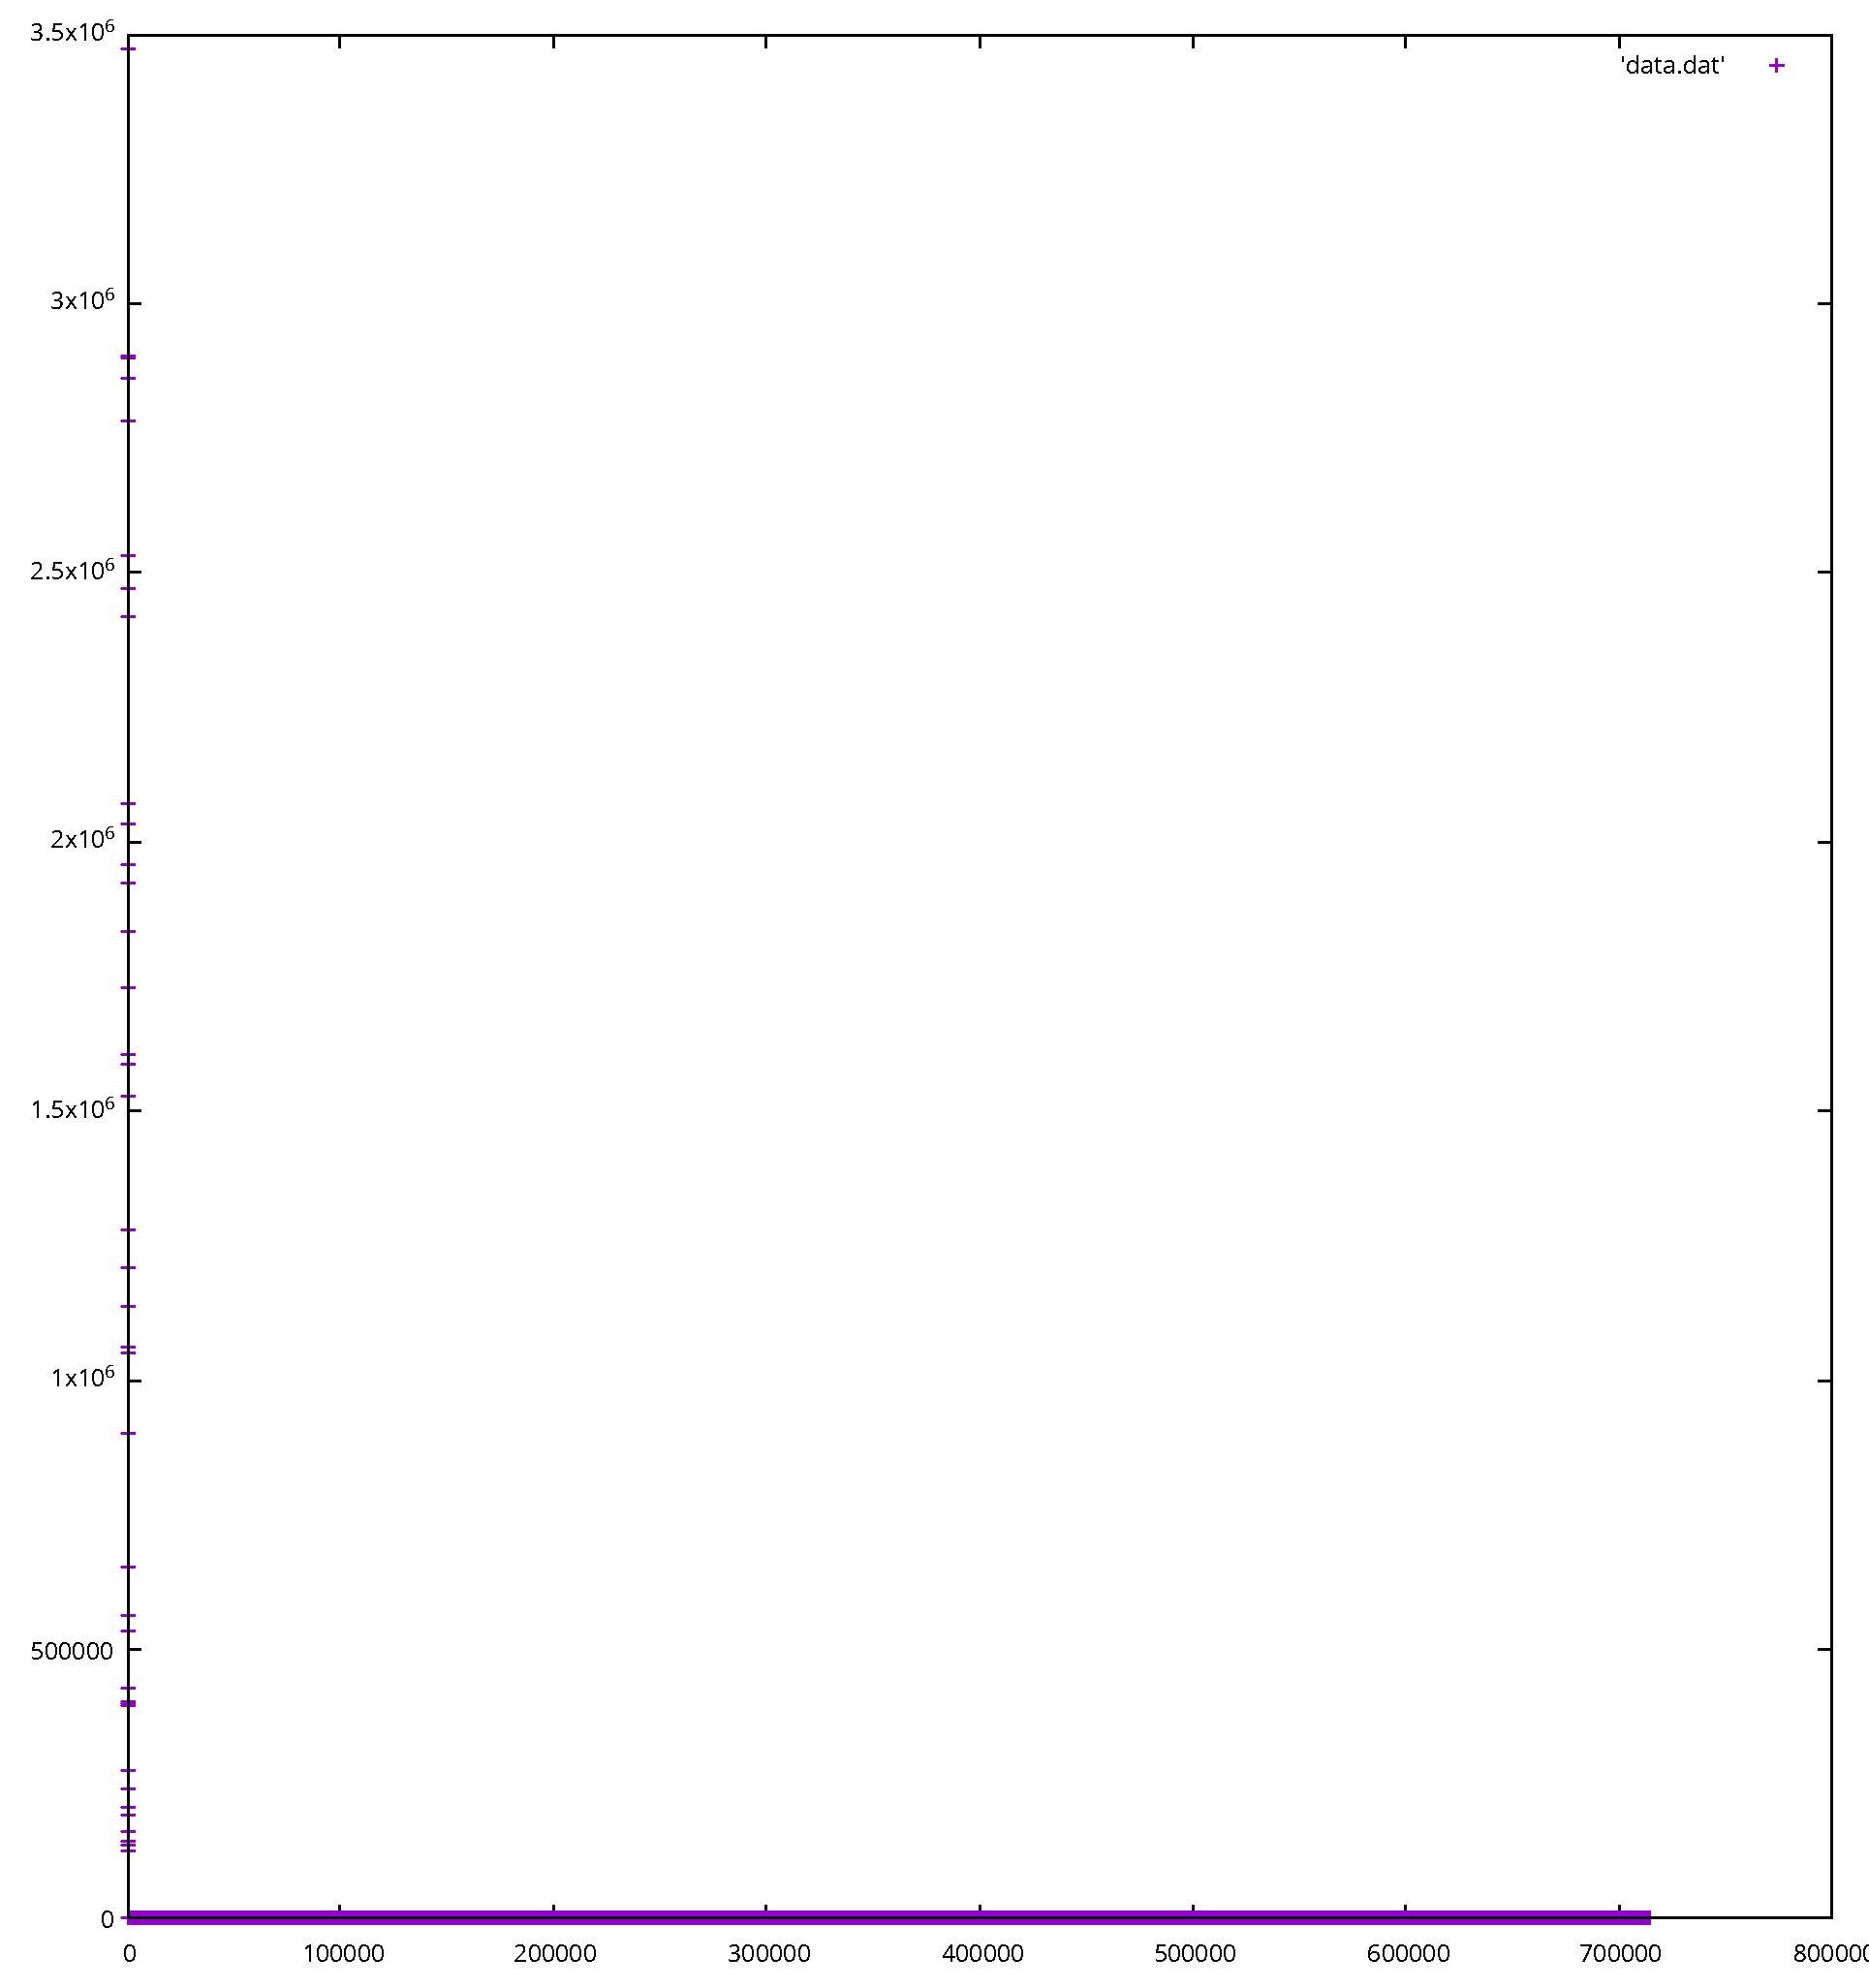
\includepdf[]{first_solution.pdf}

Como se puede puede ver, hay un completa falta de exploraci\'on al principio que nos lleva de manera precipitada a una soluci\'on. Esto es por el valor tan bajo que ten\'ia la temperatura inicial.El incrementar la temperatura lleva a un mayor porcentaje de aceptaci\'on y a una mayor exploraci\'on pero incrementa el tiempo de ejecuci\'on. Del mismo modo con el tamaño de lote/\\

Despu\'es de varios intentos fallidos estas fueron algunas de las observaciones concluidas.\\

La primera etapa de la experimentaci\'on consiste en afinar los par\'ametros. Fue mejor correr un n\'umero reducido de semillas en esta etapa, de esta manera se obtienen resultados r\'apidos y hay exploraci\'on constante, tal como la heur\'istica, el principio es el momento de intentar par\'ametros muy grandes so muy chicos. Y observando los resultados uno converge a par\'ametros m\'as \'optimos para cada caso. \\


Una vez que los resultados parecen ser favorables es entonces cuando llega el momento de correr una gran cantidad de semillas para experimentar con la probabilidad de encontrar mejores soluciones. \\

Durante la experimentaci\'on una de las observaciones encontradas es que una epsilon menor parece encontrar mejores soluciones para el caso con un mayor n\'umero de ciudades, en cambio el usar una epsilon muy reducida para el caso con menos ciudades pareci\'ia hacer que el algoritmo tardara mucho o no terminara, adem\'as de que los resultados dados no eran tan favorables. Por lo que usar $\epsilon = 0.0001$ para 150 ciudaded y $\epsilon = 0.002$ para 40 ciudades, parece ser la manera de encontrar soluciones m\'as \'optimas. \\


Como el uso de la her\'istica de temperatura incial fue implementada ya por el final, llev\'o a que una parte del tiempo de experimentaci\'on se haya usado para manualmente calcular una temperatura indicada para el caso general.  \\

Dentro del algoritmo de temperatura inicial , el cambiar a un porcentaje de aceptaci\'on mayor parece permitir una mayor exploraci\'on lo que genera una mayor cantidad de resultados factibles sacrificando tiempo de ejecici\'on.\\

Del mismo modo la temperatura inicial generada por el algoritmo para el caso de 40 ciudades es m\'as grande que la generada para 150 ciudades. En el caso de 40  el rango de tempraturas generadas era de 200,000-300,000 , sin embargo , para el de 150 ciudades el rango era de 120,000-150,000 aproximandate. Este patr\'on igual se puede ver al correr la instancia de 200 ciudades, el cual generaba temperaturas dento de un rango de 60,000-90,000. \\


Esto parece contraintuitivo, pero si consideramos que  casos con menores ciudades es m\'as r\'apido encontrar soluciones factibles por lo que tenemos un mayor rango de exploraci\'on, en cambio el encontrar soluciones factibles con un mayor n\'umero de ciudades es m\'as dif\'icil, as\'i que una vez cuando el algoritmo encuentra mejores soluciones entonces es mejor permanecer en un rango amenorado .\\

Del mismo modo el porcentaje de de soluciones factibles parece bajar al incrementar el n\'umero de ciudades, ya que cada vez se vuelve m\'as dif\'icil encontrar soluciones factibles. Con 40 ciudades el porcentaje de soluciones factibles oscilaba entre 80 -90\% , en cambio con 150 ciudades estaba en 70-80\% , y con 200 ciudades 40-50\% aproximadamente.\\

Probablemente el hecho de combinar el generar una temperatura incial con un mayor porcentaje de aceptaci\'on y tener una epsilon con un valor bastante bajo, llev\'o a que durante la exploraci\'on encontrara un camino o direcci\'on  favorable y se epecializara de manera decisiva por el final hasta llegar a la soluci\'on m\'as m\'inima. Esto igual se puede ver en el n\'umero de iteraciones del algoritmo de barrido, para 40 ciudades donde la epsilon era myor el barrido corre varias veces, en cambio para las soluciones de 150 como epsilon es menor y las soluciones est\'as m\'as cerca del m\'inimo local, el barrido solo corre unas cuantas veces.

\subsection*{Gr\'aficas de las mejores soluciones}
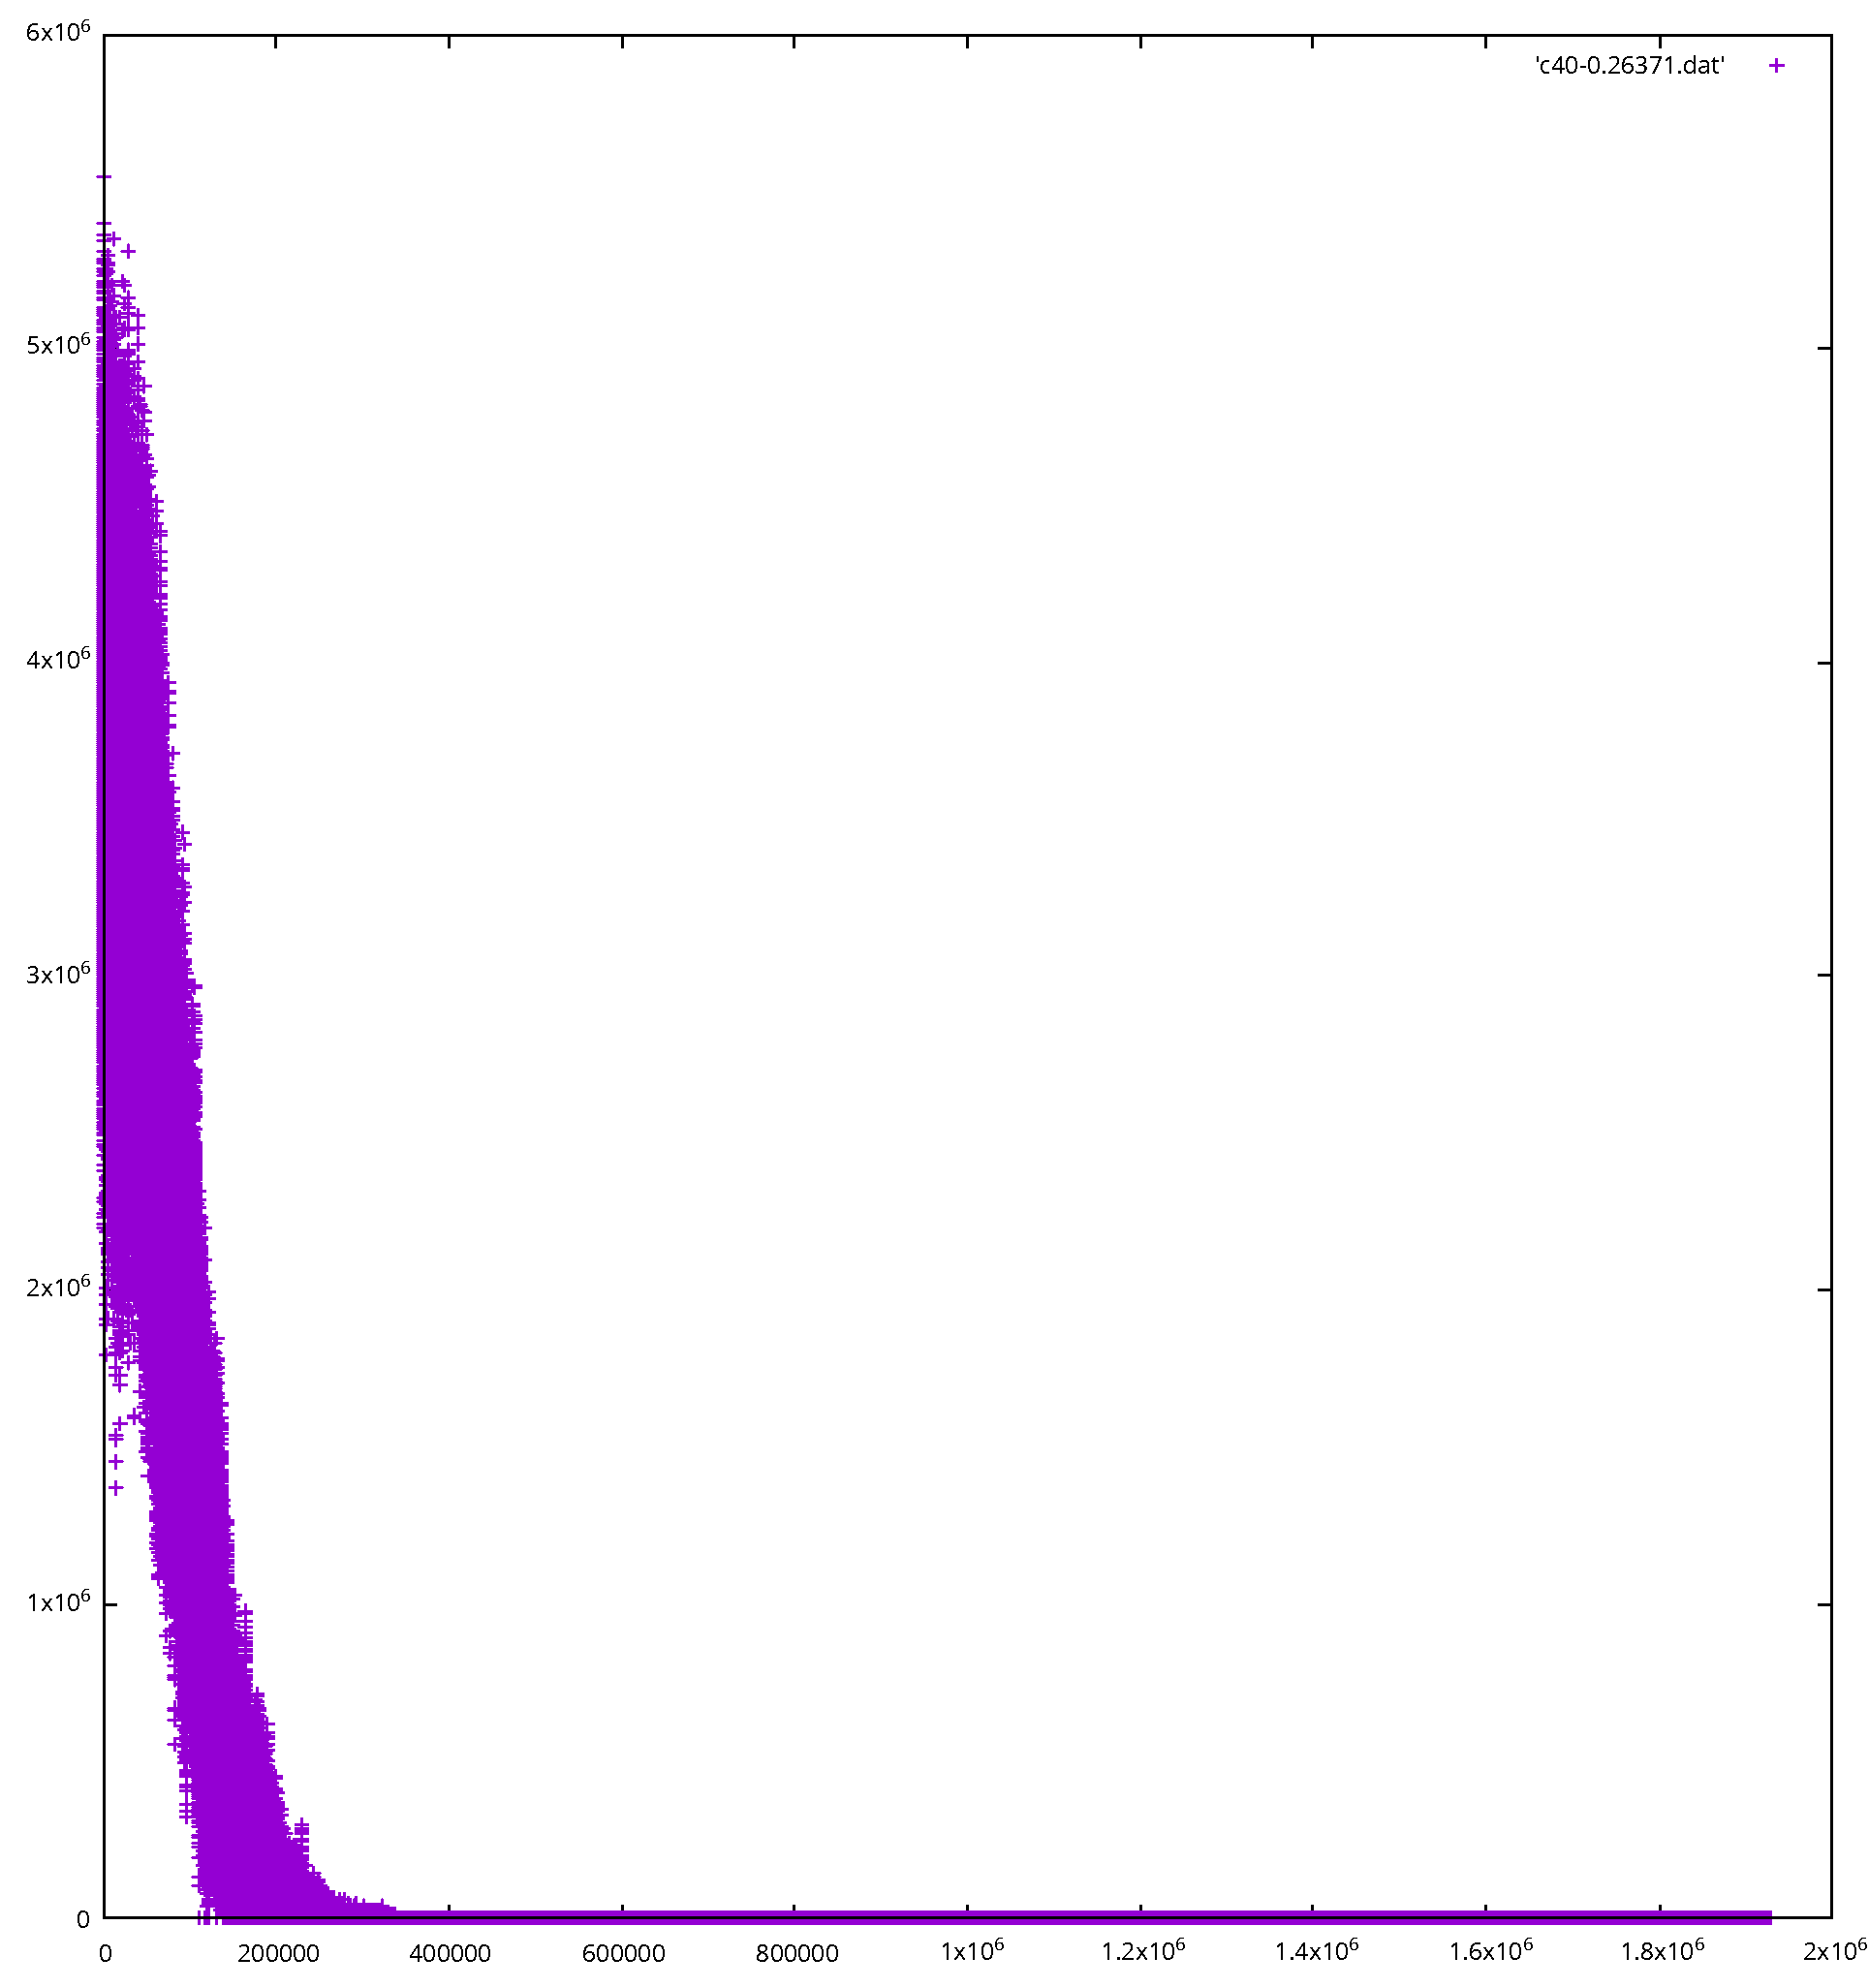
\includepdf[]{c40-0.26371.pdf}

%\subsection*{Gr\'afica de la soluci\'on para 150 ciudades}
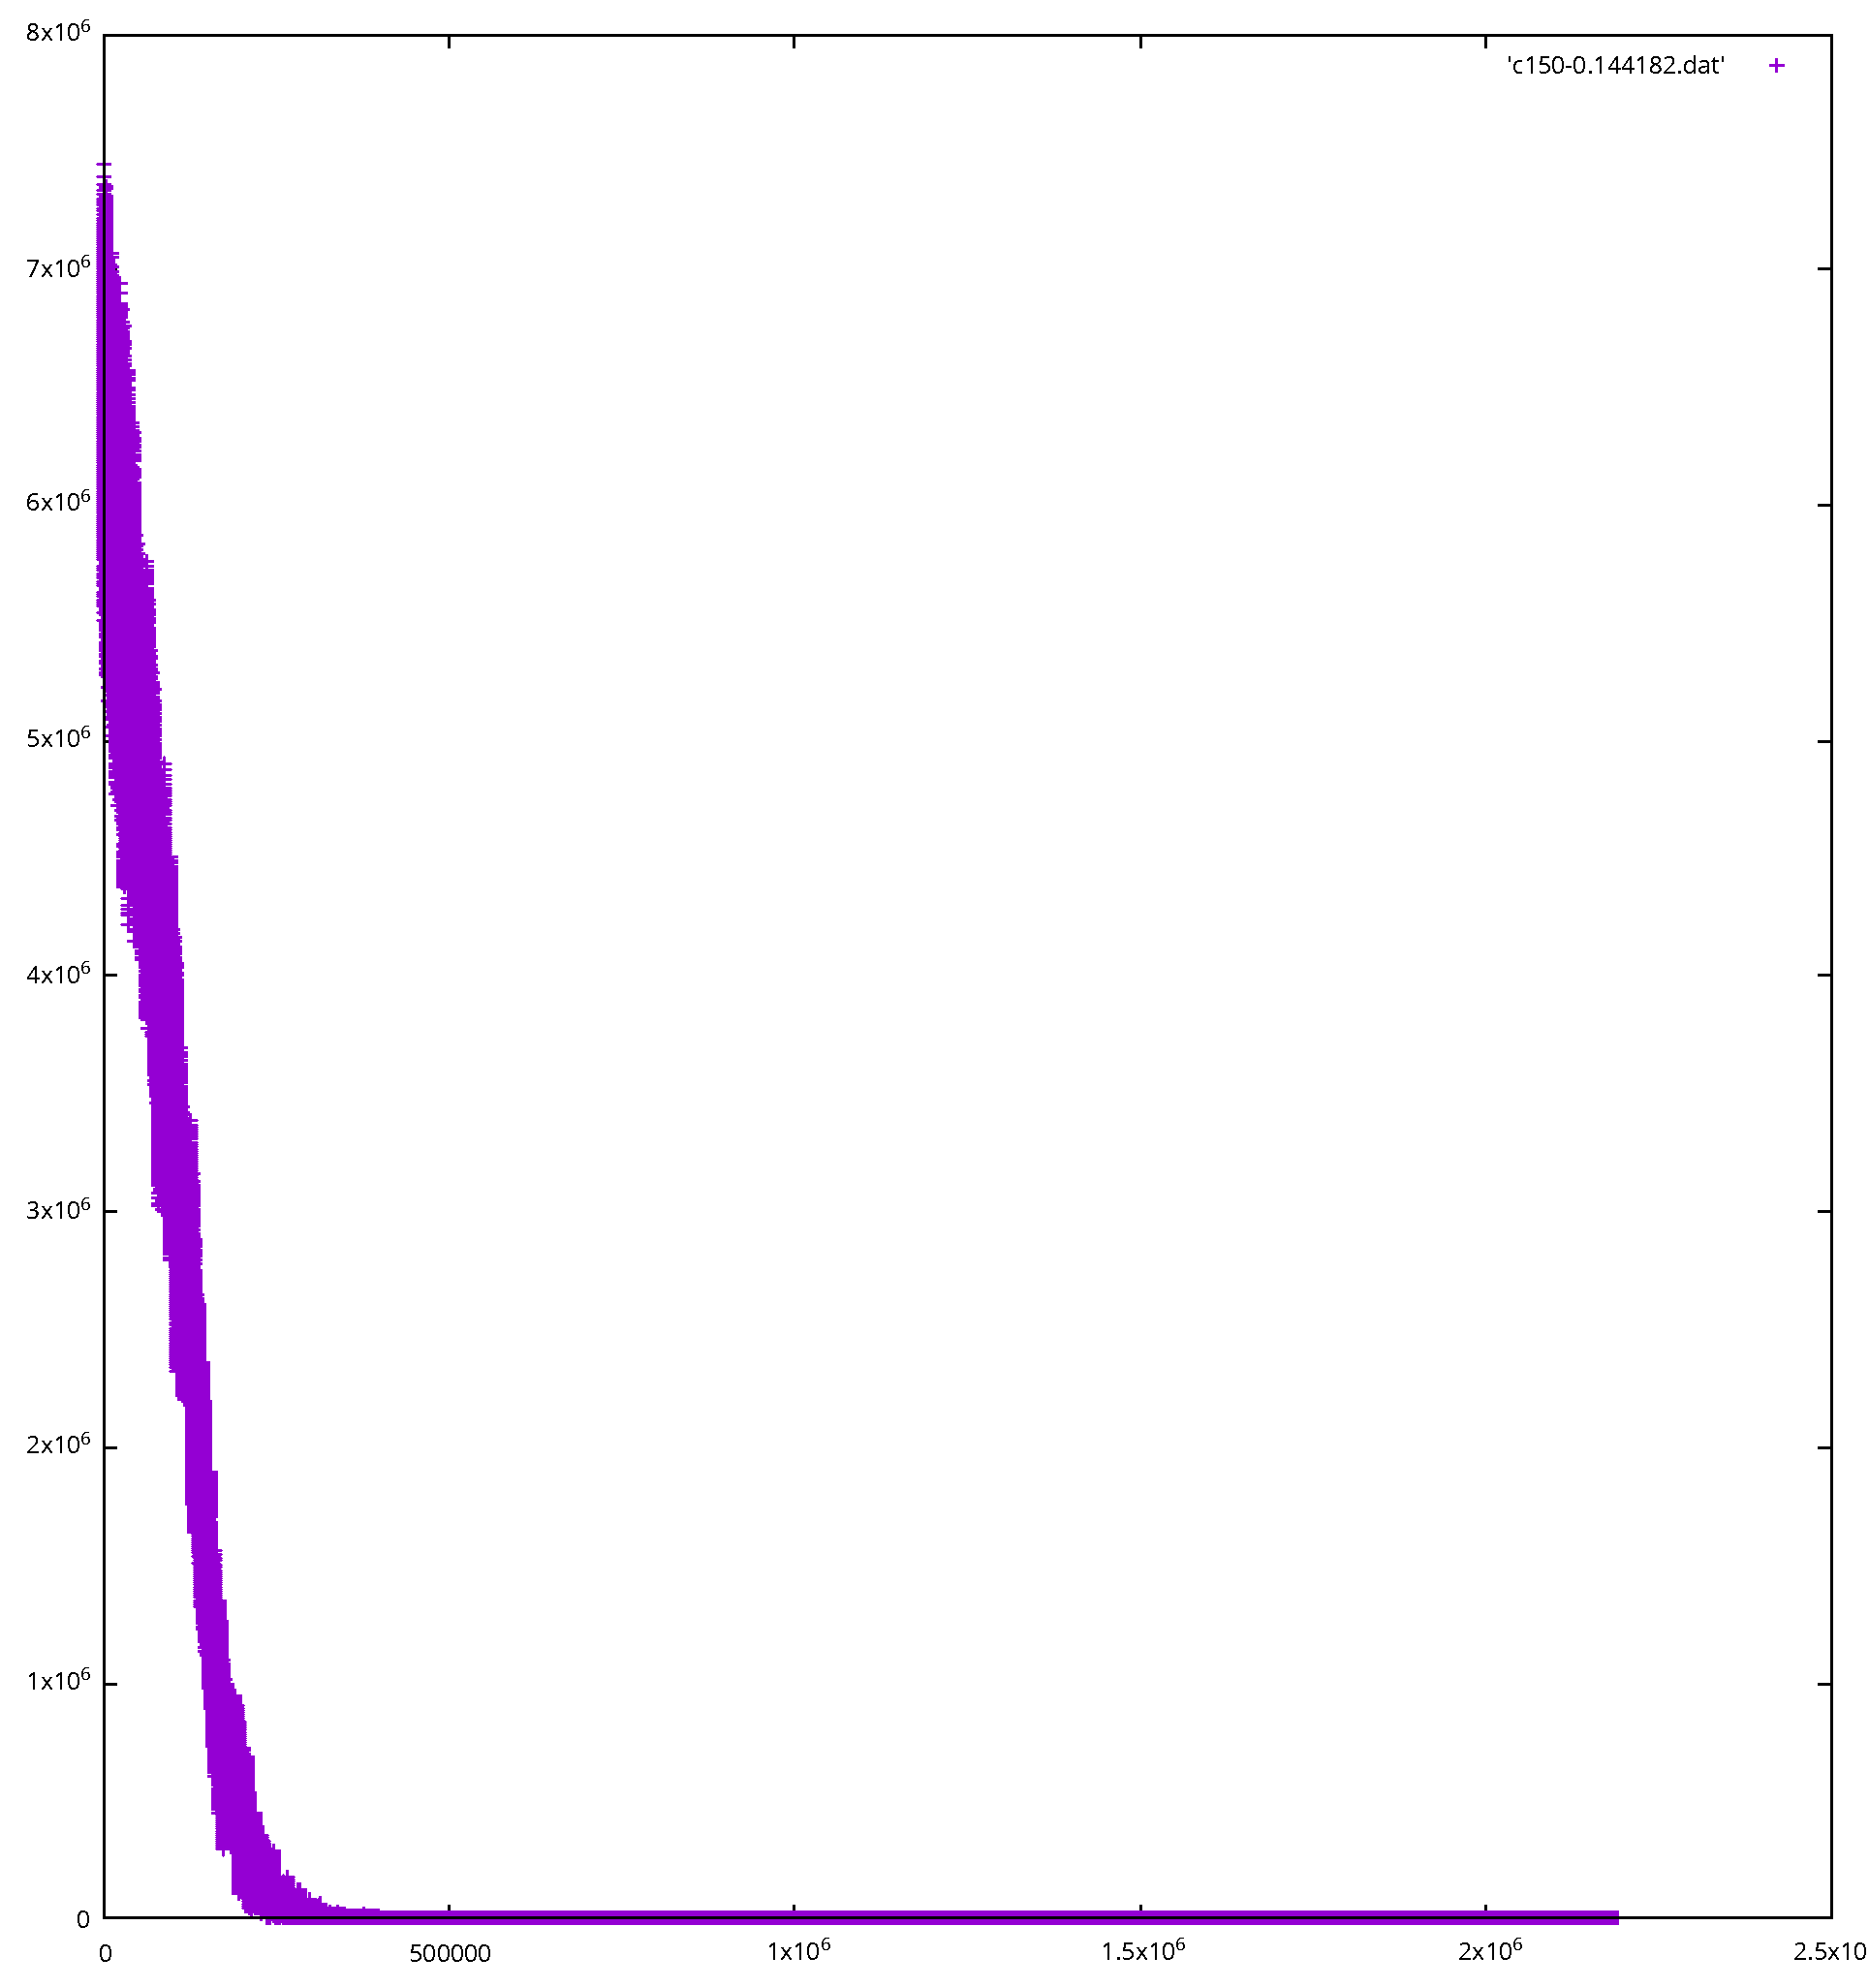
\includepdf[]{c150-0.144182.pdf}
\section*{Reproducir los resultados}
Una parte importante y la raz\'on por la que se usan semillas al generar los n\'umeros aleatorios, es que los resultados encontrados sean reproducibles.\\

Esta es la lista de variables usadas para obtener estos resultados, y c\'omo reproducirlos.

\subsection*{Para el caso con 40 ciudades}
Las variables usadas fueron
\begin{itemize}
\item Evaluaci\'on : 0.2637132755109184
\item El camino:
  \begin{align*}
    &[979, 493, 329, 163, 172, 496, 815, 657, 168, 1, 656, 2, 653, 490, 654, 7, 816, 982, 332, 820,\\
    &981, 333, 3, 165, 6, 5, 978, 817, 4, 489, 492, 491, 984, 331, 164, 327, 980, 186, 483, 54]
  \end{align*}
  
\item Epsilon : 0.002
\item Phi : 0.98
\item Tamaño de lote : 1000
\item Semilla de vecinos aleatorios : 16214040050592208640
\item Semilla para generar la soluci\'on inicial : 16042267250931732492
\end{itemize}
Para poder correr esta instancia, ejecutar lo siguiente desde la l\'inea de comandos.
\begin{lstlisting}
  cd target/release
  ./simulated_annealing --cities40 -e 0.002 --neigh 16214040050592208640
                        --init 16042267250931732492
\end{lstlisting}
% % (0.2637132755109184, [979, 493, 329, 163, 172, 496, 815, 657, 168, 1, 656, 2, 653, 490, 654, 7, 816, 982, 332, 820, 981, 333, 3, 165, 6, 5, 978, 817, 4, 489, 492, 491, 984, 331, 164, 327, 980, 186, 483, 54], 16214040050592208640, 16042267250931732492)
% 11613177925935108993, 8480295797754924014)
% % neighbor seed , initial_solution seed
\subsection*{Para el caso con 150 ciudades}
\begin{itemize}
\item Evaluaci\'on : 0.14418250861220022196
\item El camino:
  \begin{align*}
    &[54, 652, 1075, 483, 171, 77, 183, 346, 75, 821, 512, 179, 671, 16, 520, 186, 190, 675, 340, 502,\\
    &151, 828, 12, 1038, 339, 826, 444, 17, 164, 11, 501, 25, 492, 491, 499, 347, 489, 4, 174, 817,\\
    &23, 176, 668, 352, 978, 5, 6, 988, 165, 3, 981, 990, 333, 991, 351, 185, 22, 676, 665, 173, 2,\\
    &656, 184, 815, 172, 182, 496, 19, 505, 168, 508, 986, 9, 1, 829, 657, 663, 661, 832, 667, 507,\\
    &653, 344, 490, 654, 26, 820, 345, 332, 181, 14, 982, 187, 816, 678, 823, 7, 673, 163, 329, 509,\\
    &493, 979, 837, 995, 984, 1003, 349, 331, 662, 8, 999, 674, 334, 343, 510, 660, 20, 680, 825,\\
    &500, 985, 504, 511, 327, 670, 350, 840, 336, 297, 980, 191, 822, 1001, 74, 166, 658, 666, 818,\\
    &655, 819, 330, 1073, 169, 1037, 326, 328, 167, 495, 494]
  \end{align*}
  
\item Epsilon : 0.0001
\item Phi : 0.98
\item Tamaño de lote : 1000
\item Semilla de vecinos aleatorios : 11613177925935108993
\item Semilla para generar la soluci\'on inicial : 8480295797754924014
\end{itemize}
Primero se debe de cambiar la siguiete l\'inea de c\'odigo dentro del archivo \texttt{sa.rs}
\begin{lstlisting}
  105 let mut batch_average = 1000000000.0;
\end{lstlisting}

despu\'es, ejecutar lo siguiente desde la l\'inea de comandos.
\begin{lstlisting}
  cd target/release
  ./simulated_annealing --cities150 --neigh 11613177925935108993
                        --init 8480295797754924014
                      \end{lstlisting}



%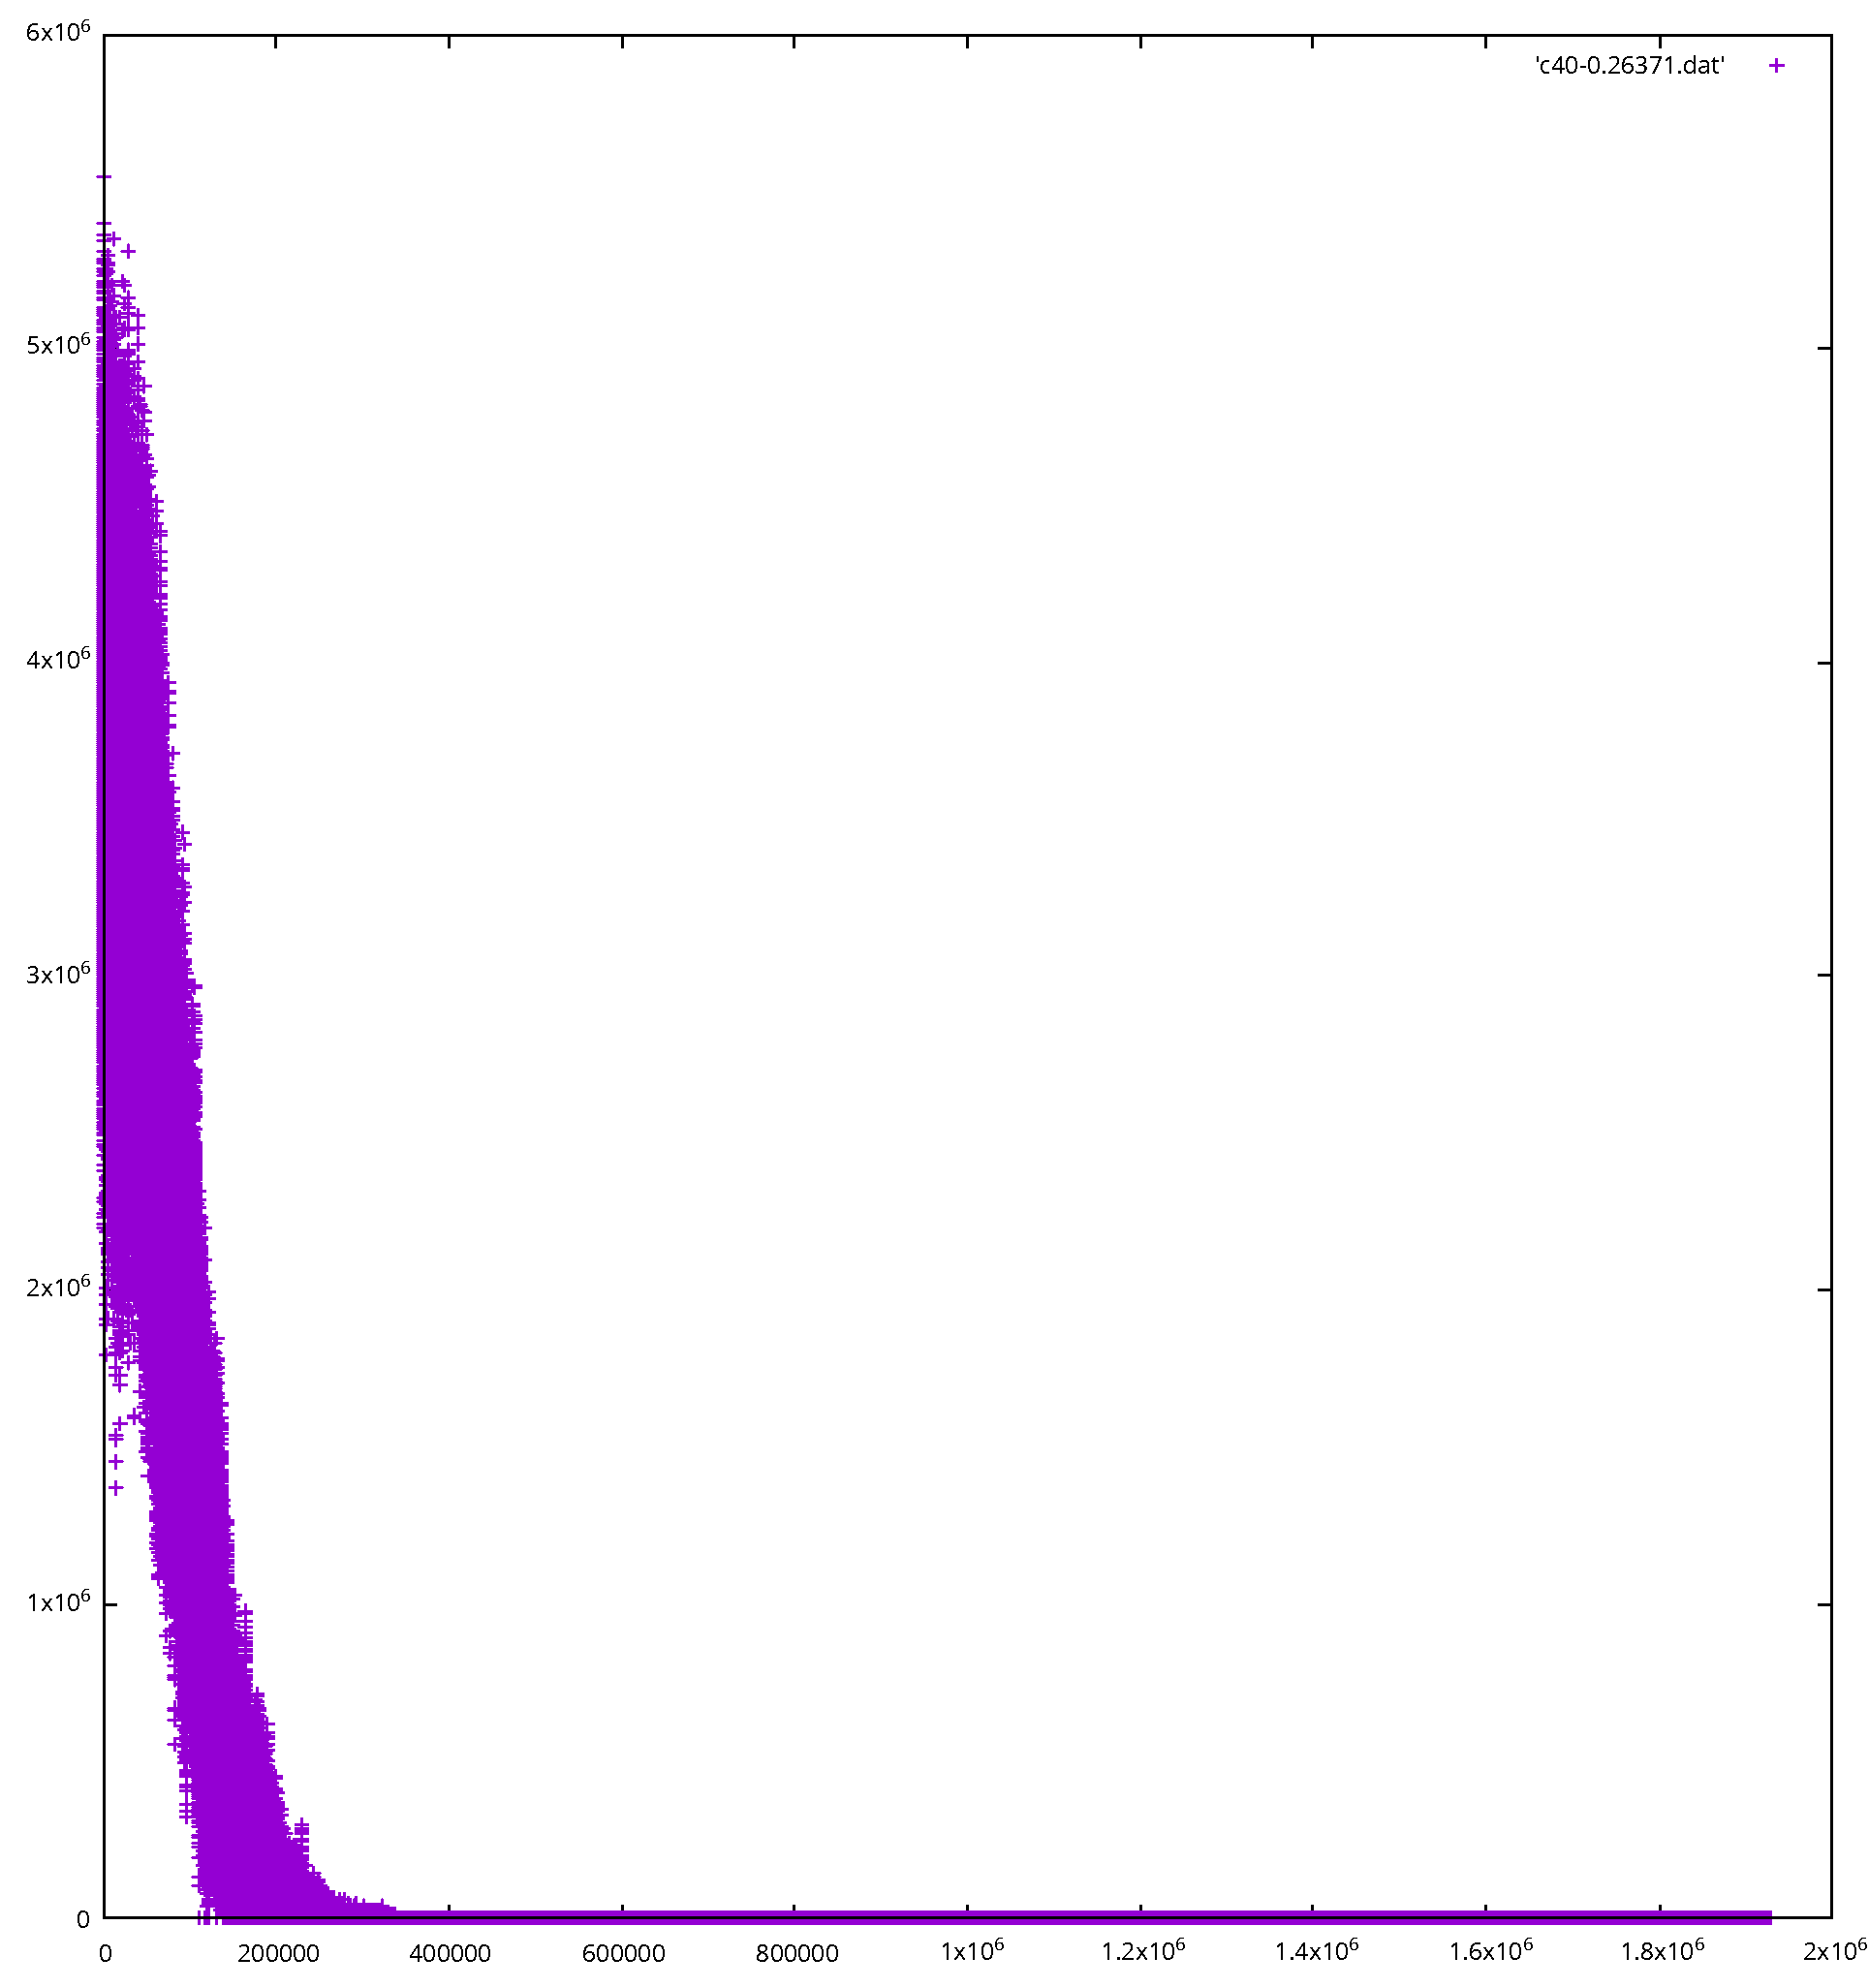
\includepdf[]{c40-0.26371.pdf}
\section*{Conclusiones}
Incluso para un sistema relativamente chico la importancia de la planeaci\'on y el diseño  sigue siendo igual de importante, reduce el tiempo de implementaci\'on y elimina el tiempo gastado por refactorizaci\'on, del mismo modo con las pruebas unitarias.   \\

Aunque la experimentaci\'on sea la \'ultima etapa del proyecto, este debe abarcar la mayor parte del tiempo, ya que la funcionalidad de la her\'istica depende de los par\'ametros usados.

\bibliography{citations}{}
\bibliographystyle{plain}
\end{document}